\documentclass[UTF8]{standalone}
\usepackage{tikz}
\usetikzlibrary{positioning}
\usepackage{ctex}

\begin{document}
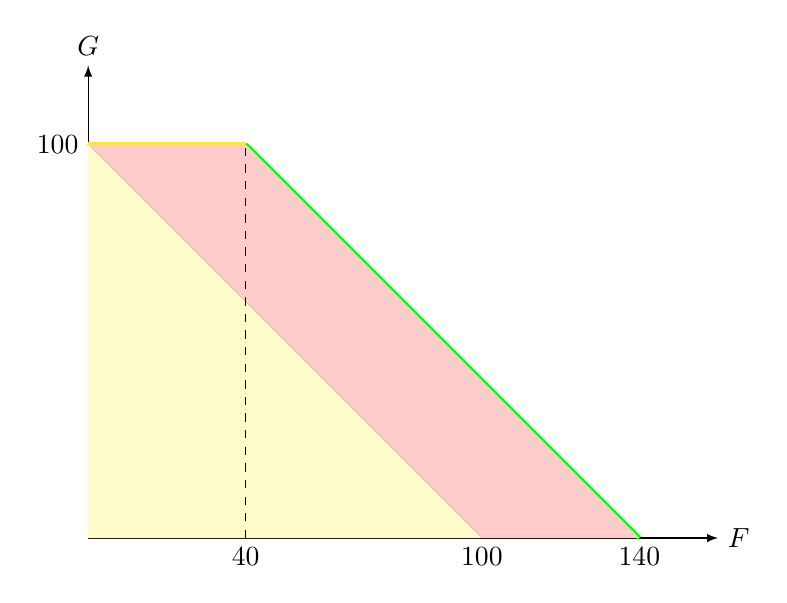
\begin{tikzpicture}
    \draw[-latex] (0,0) -- (8,0) node[right] {$F$};
    \draw[-latex] (0,0) -- (0,6) node[above] {$G$};

    \draw[domain=0:5, thick] plot (\x, {-\x+5});
    \node[left] at (0,5) {$100$};
    \node[below] at (5,0) {$100$};

    \draw[domain=0:2, ultra thick, yellow] plot (\x, {5});
    \draw[domain=2:7, ultra thick, green] plot (\x, {-\x+7});
    \node[below] at (7,0) {$140$};

    \fill[yellow!20] (0,0) -- (0,5) -- (5,0) -- cycle;
    \fill[red!20] (0,5) -- (5,0) -- (7,0) -- (2,5) -- cycle;

    \draw[dashed] (2,0) -- (2,5);
    \node[below] at (2,0) {$40$};

    
\end{tikzpicture}
\end{document}